\chapter{Formalization}
\label{sec:formalization}

\section{Intermediate Representation: CCDFG}

In order to formalize and prove the correspondence between pipelined
and unpipelined IRs, a first step is to define a formalization of the
IRs themselves.  We call our formalization of IRs {\em Clocked Control
  Data Flow Graph} (CCDFG).  An informal description of CCDFG has been
provided before~\cite{rhcxy:atva-09}.  It can be best viewed as a
traditional control/data flow graph used by most compilers, augmented
with a schedule. Control flow is broken into basic blocks.
Instructions are grouped into microsteps which can be executed
concurrently.  A scheduling step is a group of microsteps which can be
executed in a single clock cycle. The state of a CCDFG at a particular
microstep is a list of all the variables of a CCDFG with their
corresponding values.

The semantics of CCDFG require a formalization of the
underlying language used to represent the individual
instructions in each scheduling step.  The underlying
language we use is the LLVM~\cite{llvm}.  It is a popular
compiler infrastructure for many behavioral synthesis tools
and includes an assembly language front-end.  At the point
of this writing we support a limited subset of LLVM, which
however is sufficient to handle all the designs we have
seen.  Instructions supported include assignment, load,
store, bounded arithmetic, bit vectors, arrays, and pointer
manipulation instructions.  We define the syntax of each
type of statement by defining an ACL2 predicate.  For
example, in our syntax, an assignment statement can be
expressed as a list of a variable and an
expression.

An expression can further be of multiple types, %\eg, 
load
expression (loading the value of a variable from memory), add
expression (addition of two variables), xor expression (xor of two variables)
etc., where each expression includes the operation applied to the
appropriate number of arguments.

We provide semantics to these instructions through a
state-based operational formalization as is common with
ACL2.  We define the notion of a CCDFG state, which includes
the states of the variables, memory, pointers, etc.  Then we
define the semantics of each instruction by specifying how
it changes the state.  Thus, for an assignment statement we
will have a function {\tt execute-assignment} that specifies
the effect of executing the assignment statement on a CCDFG
state.

Defining the semantics of most supported statements is
straightforward, with one exception.  The exception is the
so-called ``$\phi$-construct'' available in LLVM.  A
$\phi$-construct is a list of $\phi$-statements.  A
$\phi$-statement is $v := \phi [\sigma, bb1] [\tau, bb2]$,
where $v$ is a variable, $\sigma$ and $\tau$ are
expressions, and $bb1$ and $bb2$ are basic blocks: if it is
reached from $bb1$ then it is the same as the assignment
statement $v := \sigma$; if reached from $bb2$, it is the
same as $v := \tau$; the meaning is undefined otherwise. The
construct is complex since the effect of executing this
statement on a CCDFG state $s$ depends not only on the state
$s$ but also on how $s$ is reached by the control flow.
Unfortunately, $\phi$-statements are required in loop designs ---
they are used to evaluate the value of loop carried dependencies.
Consequently, the complexity induced
by this instruction cannot be avoided.

\section{Correctness of Loop Pipelining}
%A behavioral synthesis tool automatically generates a RTL design from an ESL design through a series of
%transformations. Pipelining a loop is a critical
%transformation in behavioral synthesis.

For the purposes of this paper, a {\em pipelinable loop} is
a loop with the following restrictions~\cite{hrx:dac-12}:
\begin{enumerate}
\item no nested loop;
\item only one $Entry$ and one $Exit$ block; and
\item no branching between the scheduling steps.
\end{enumerate}

{\bf Discuss with Sandip Sir}: We should mention that there is only one conditional branch and one unconditional branch related to loop,
others can be handle via previous compiler transformations. Also, there is only one phi statement. 

These restrictions are not meant to simplify the problem, but reflect
the kind of loops that can be actually pipelined during behavioral
synthesis.  For instance, synthesis tools typically require inner
loops to have been fully unrolled (perhaps by a previous compiler
transformation) in order to pipeline the outer loop.

\begin{figure}
\begin{center}
\begin{tabular}{ccc}
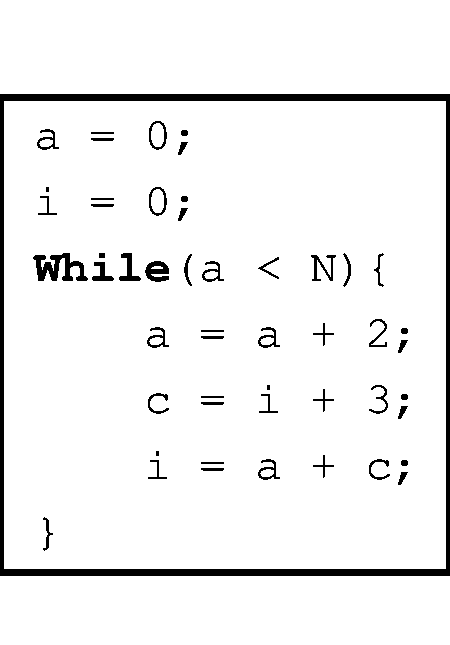
\includegraphics[height=1.6in]{fig-proposal/C-code}
&
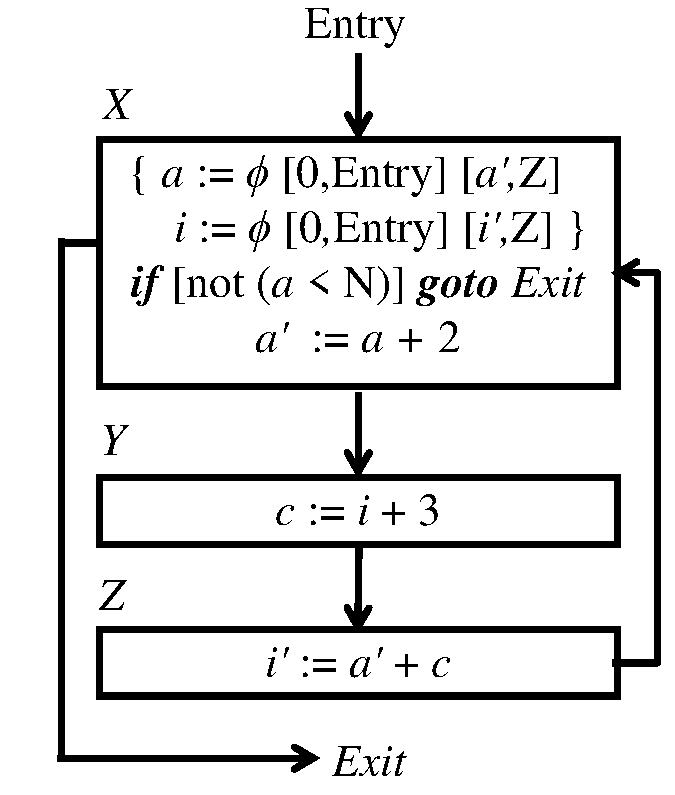
\includegraphics[height=1.6in]{fig-proposal/seq-ccdfg-1}
&
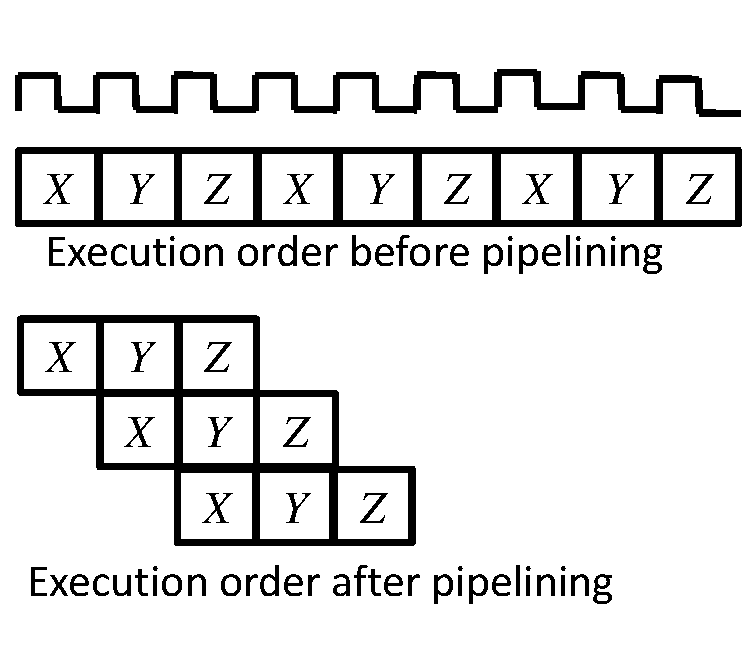
\includegraphics[height=1.6in]{fig-proposal/pp-clock-cycles}
\\
(a) & (b) & (c)
\end{tabular}
\end{center}
\caption{(a) Loop in C; (b) Loop CCDFG before pipelining ({\bf Note for Disha: create a better figure. Discuss with Zhenkun}) ; (c) Pipelining increases throughput}
\label{fig:high-level-synthesis}
\end{figure}

Figure~\ref{fig:high-level-synthesis}(a) illustrates the C
code (ESL description) for a loop.  The C code does not have
a schedule or the concept of a clock cycle.
Figure~\ref{fig:high-level-synthesis}(b) shows CCDFG of the
sequential loop just before loop pipelining. The loop has
three scheduling steps: $X$, $Y$ and $Z$.  The scheduling
step before the loop is $Entry$ and after the loop is
$Exit$. Note that there is a $\phi$-statement in the
first scheduling step of the loop.  This $\phi$-statement
accounts for those variables whose values are dependent on
the variables evaluated in a previous iteration.

Behavioral synthesis tools use complicated heuristics and aggressive scheduling strategies to
find an optimized pipeline interval (clock cycles after which a new iteration can be started such that there are no data hazards). One iteration of the sequential design takes three
clock cycles. Observe in Figure~\ref{fig:high-level-synthesis}(c) that with the pipeline interval of one, the three iterations of the pipelined loop
take five clock cycles as opposed to nine clock cycles in the sequential loop.
Loop pipelining reduces the number of clock cycles required to execute the loop, hence this transformation is used by synthesis tools to increase throughput and reduce overall latency.

%% Since, reasoning about execution becomes difficult if we have to
%% always keep track of the previous scheduling step, we treat the first
%% iteration of the sequential CCDFG {\em seq-pre-loop} as a separate
%% iteration than the rest of the iterations {\em seq-loop}.  Infact, the
%% first step of our pipelining algorithm is to unroll the loop once and
%% replace $\phi$-construct by corresponding assignment statements based
%% on the previous scheduling steps.

%% \subsection{Correctness Statement}
%% \label{subsec:correctness-defn}

%% IMPORTANT : take a look again, if we want to keep all iterations same, we can start from k = 0

 \smallskip
\noindent {\textbf {Correctness Statement:}}
Let $L$ be a loop in CCDFG $C$, and let $L_{\alpha}$ be the
pipelined implementation generated by a pipeline algorithm using
pipeline parameters $\alpha$.  Let $V$ be the set of
variables in $L$, and $U$ be the set of all
variables in $C$.  Suppose we execute $L$ and $L_{\alpha}$
from CCDFG states $s$ and $s'$ respectively, such that for
each variable $v\in V$, the value of $v$ in $s$ is the same
as that in $s'$, and suppose that the state on termination
are $f$ and $f'$ respectively.  Then (1)~for any $v\in V$,
the value of $v$ in $f$ is the same as that in $f'$, and
(2)~for any $v\in(U\backslash V)$, the value of $v$ in $f'$
is the same as that in $s'$.

\medskip
\noindent
{\em Remark:} Condition (2)
ensures that variables in $C$ that are not part of the loop
are not affected by $L_{\alpha}$.  The value of any new
variables introduced by the algorithm in $f'$ are irrelevant since they are not accessed
subsequently.


%% Important: Ask Sandip: How are we accounting for condition 2 in our correctness statement ??? Am I missing something??

%\begin{quote}
%Let $L$ be a loop in CCDFG $C$, and let $L_{\alpha}$ be the
%pipelined loop CCDFG. Let $V$ be the set of
%variables mentioned in $L$, and $U$ be the set of all
%variables in $C$.  Suppose we execute $L$ and $L_{\alpha}$
%from CCDFG states $s$ and $s'$ respectively, such that for
%each variable $v\in V$, the value of $v$ in $s$ is the same
%as that in $s'$, and suppose that the state on termination
%are $f$ and $f'$ respectively.  Then (1)~for any $v\in V$,
%the value of $v$ in $f$ is the same as that in $f'$, and
%(2)~for any $v\in(U\backslash V)$, the value of $v$ in $f'$
%is the same as that in $s'$.
%\end{quote}
%\noindent
%{\em Remark:} Condition (2) is the {\em frame rule} which
%ensures that variables in $C$ that are not part of the loop
%are not affected by $L_{\alpha}$. The algorithm introduces
%additional variables, eg, {\em shadow variables}
%(cf. Section~\ref{sec:proof}).  The values of these
%variables in $f'$ are irrelevant since they are not accessed
%subsequently.



%\medskip
%\noindent{{\bf CCDFG :}} Formalizing the correctness
%statement entails defining the semantics of CCDFG.  A CCDFG
%is a control/data flow graph augmented
%with a schedule.
%Control flow is broken into basic blocks.  Instructions in a
%basic block are grouped into {\em microsteps} that are
%executed concurrently.  A schedule is a grouping of
%microsteps which can be completed within one clock cycle.
%The instruction language we support is a subset of
%LLVM~\cite{llvm} which is a front-end for many behavioral
%synthesis tools~\cite{autoesl,xpilot,legup}; we support
%assignment, load, store, bounded arithmetic, bit vectors,
%arrays, and pointer manipulations.  As is common with ACL2,
%we use a state-based operational semantics.  Assigning
%meanings to most instructions is standard; one exception is
%the $\phi$-statement ``{\tt v := phi [$\sigma$ bb1] [$\tau$
 %   bb2]}''.  If reached from basic block {\tt bb1}, it is
%the same as the assignment statement {\tt v := $\sigma$}; if
%reached from {\tt bb2}, it is the same as {\tt v := $\tau$};
%the meaning is undefined otherwise.  Reasoning about
%$\phi$-statement is complex since after its execution from
%state $s$, the state reached depends not only on $s$ but
%previous basic block in the history. However,
%We need to
%handle it since it is used extensively to implement loop
%tests.  Indeed,
%A key step in loop pipelining is
%$\phi$-elimination, \viz, unrolling the loop once and
%replacing the $\phi$-statement with assignment statements
%(cf. Fig.~\ref{fig:loop}).








